\section{Discussion}
\label{sec:discussion}

\subsection{What is different about a millimetre technosignature search}
\label{sec:mmdifferent}

This experiment's most transferable result is not the non-detection but
a measurement of what limits a carrier search at these wavelengths. It is not
depth: the power a transmitter must radiate to cross the threshold here is a median
$\EirpNinetySysMedA$\,W per system, and more power buys nothing at a
frequency the archive never tuned to or never returned to. That
inherited coverage sets the limit. Molecular-line confusion is a different
matter: it costs bandwidth, and it decides how a crossing is disposed of once
one is found.

\emph{Line emission, and not interference, is the astrophysical false
positive here.}
Catalogued molecular transitions, almost all of them carbon monoxide, account
for \EvNAttrQp{} of the \EvNCrossQp{} crossings in quality-passing data, and
no crossing in this survey is attributed to interference
(Appendix~\ref{app:rfi}). \LnAttrSupp{} of those attributions carry support
beyond the frequency match -- a second transition of the same species,
catalogued gas on the sightline, or the crossing's own recurrence -- while
\LnAttrCoincWord{} rest on the coincidence alone, which leaves them
consistent with molecular emission and not identified as it. The
attributed crossings include the strongest events in the quality-passing
data, but they are
not the commonest: of the \EvNUnattrQp{} unattributed crossings the \CeObs{}
of the primary census are no more numerous than the control positions of
their own fields predict
(\S\ref{sec:trigunif}), so chance at a trigger of \StageNullTrig{} is enough
to account for most crossings by number while line emission accounts for the
ones that stand out.
\DiscFpWin{} of the \DiscFpOfFlags{} windows that reached the spatial stage
are disc or interstellar carbon monoxide, all but one the resolved disc of
$\beta$~Pictoris and the exception a cloud along the sightline to
HD~48370. The remedy that works is a velocity-space mask evaluated in each star's
own rest frame, and \S\ref{sec:bpicval} gives what it costs in
bandwidth.

\emph{Spatially extended emission is the second discriminant, and it has no
analogue at centimetre wavelengths.} A line filling the primary beam raises
the star and the control annulus together instead of cancelling, so the
spatial statistic loses power exactly where circumstellar gas is brightest:
$\beta$~Pictoris shows the benign face, its circumstellar carbon monoxide
recovered by the same search (\S\ref{sec:bpicval}), and HD~48370 the other,
its emission an interstellar cloud and not a disc
(Appendix~\ref{app:linemask}), lying near a band edge, and that one window
contributing \VnEdgeDomPct{} per cent of every near-edge threshold exceedance
in the survey. Pooled, the near-edge rate is $\times\VnEdgeRatio$ the
interior rate; without that window it is $\times\VnEdgeNoDomRatio$, and on a
held-out half $\times\VnEdgeHalfCleanRatio$
($\pv{\VnEdgeHalfCleanP}$). That near-edge excess is
one interstellar cloud, so no edge correction is
applied to any limit.

An illustrative engineering benchmark fixes the scale these limits reach. A
\BenchDiam\,m dish radiating \BenchPowerMW\,MW at \BenchFreqGHz\,GHz with an
aperture efficiency of \BenchEta{} has a directive gain
$G=\eta(\pi D\nu/c)^{2}=\BenchGain$ and so an EIRP of $\BenchEirp$\,W, above
the single-epoch crossing limit of \BenchNSysA{} of the \NSysClassA{} Class~A
systems. The same gain makes its beam $\Omega=4\pi/G=\BmOmegaSr$\,sr,
illuminating $\BmSkyFrac$ of the sky with a half-power width of \BmArcsec{}
arcsec, and EIRP is not transmitter power -- the same megawatt radiated
isotropically would be $10^{6}$\,W -- so these limits apply to beamed
transmitters whose beam contains the Solar System.

\emph{The channelisation is inherited.} In \ScCoarseNoDrift{} of the
\NWinB{} coarse-channel windows every drift in the grid stays inside one channel over a
whole track and in \EtaDriftBHi{} more it crosses barely one; none of them
can distinguish a drifting carrier from a stationary one, which is why the
carrier search rests on the \NWinA{} fine-channel windows. The widths on offer here run from \SzChanFinestKHz\,kHz to
\SzChanWidestMHz\,MHz, about \SzChanDexSurvey{} orders of magnitude. Set
beside the \SzChanLitHz\,Hz channels of centimetre-band carrier searches the
range becomes \SzChanDexAll{} orders (Fig.~\ref{fig:context}(b)), and
nothing in the search could choose them.

\emph{Repeat epochs turn a crossing into a testable claim, and an archive
supplies them only incidentally.} Let the \emph{confirmation coverage}
$C_{\rm conf}(\nu)$ be the number of systems toward which two execution
blocks of different observing sessions more than a day apart both cover the
sky frequency $\nu$, so
that a carrier found once there could have been sought again. It must be
stated against frequency and not as a fraction of the sample, because
repeat visits re-tune and a second epoch is of no use at a frequency it does
not cover. Its support is \CvConfGHzDay\,GHz of union bandwidth, \CvConfPctDay{} per
cent of the \CvUnionA\,GHz searched, and it falls to \CvConfGHzYr\,GHz
beyond a year. At its best, near \CvConfNuMaxDay\,GHz, it reaches
\CvConfNMaxDay{} systems (Fig.~\ref{fig:confcov}). The searched extent
is about twice the extent over which a carrier returning to its predicted
cell could have been
confirmed, and for close to half the sample the archive constrains an
intermittent emitter hardly at all, whatever its power.

\begin{figure}
\centering
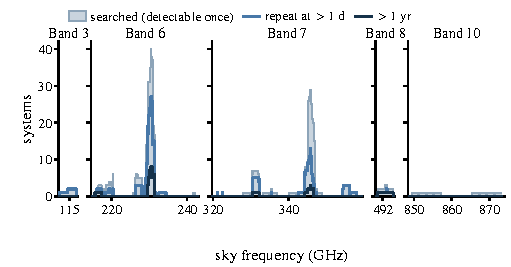
\includegraphics[width=\columnwidth]{figures/confcoverage.pdf}
%% ★ v4.26 (r25-captions): 8 printed lines -> R1 §7's limit of about six.
%% "a block of another observing session more than a day later" IS the defined
%% term \emph{separated} (Table~\ref{tab:quantities}), so naming the term is
%% both shorter and the paper's own usage.  The orbital-phase caveat is KEPT
%% here: it was dropped from Fig.~\ref{fig:classasens}'s caption, which
%% carried it as well, and this is the panel it bites hardest on.  "as in
%% Fig.~\ref{fig:covmap}" went because that caption states the same panel
%% rule in the same words.  No macro lost a citation site.
\caption{What could be searched against where a separated repeat exists.
Class~A systems against sky frequency: detectable once (grey); with a
\emph{separated} block (Table~\ref{tab:quantities}) covering it (blue);
beyond a year (dark). An accelerating carrier further needs a matching
orbital phase. One panel per populated ALMA band, width proportional to its
frequency share.}
\label{fig:confcov}
\end{figure}

\subsection{The search space this archive opens}
\label{sec:newspace}

The searches of \citet{Steffes1994} and \citet{Mauersberger1996} reached
nearby stars above about 30\,GHz at one frequency only, and the one other
millimetre search of more than a single line, \citet{Mason2025},
covered \MasonBandMHz\,MHz of Band~3 toward far more distant stars
(\S\ref{sec:intro}); Band~3 is searched here, in
\NWinBandThree{} windows down to \SurvFreqLo\,GHz including
$\beta$~Pictoris' CO $J=1\!-\!0$ control. The haystack axis of \citet{Wright2018} runs from \SttHayLoMHz\,MHz to
\SttHayHiGHz\,GHz, and this experiment covers \SttHayGHz\,GHz of it. Only
\SttHayFineGHz\,GHz of that is carrier search, because the Class~A union
spans \SurvFreqLoA--\SurvFreqHiA\,GHz, and the rest lies above the axis
altogether.

Union bandwidth overstates what that buys: different frequencies were searched
toward different numbers of stars and to very different
limits. Figure~\ref{fig:covmap} gives instead the number of independent systems
that would have yielded a recovery at ninety per cent completeness, against sky
frequency and transmitter power. At an EIRP of $\CovEirpRefTex$\,W the covered frequency falls to
\CovUnionAtRef\,GHz, which is \CovFracAtRef{} per cent of the union. It
reaches \CovNSysAtRef{} systems, and \CovNMaxAtRef{} at the best-covered
frequency near \CovNuMaxAtRef\,GHz. With no limit on power at all that
frequency reaches \CovNMaxFull{} of the \NSysClassA{} systems, and half the
sample is reached only above $\CovEirpHalf$\,W.

\begin{figure}
\centering
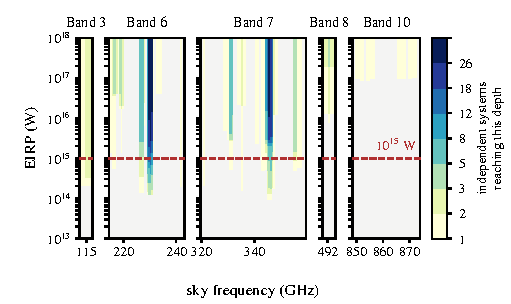
\includegraphics[width=\columnwidth]{figures/completeness_map.pdf}
%% ★ v4.26 (r25-captions): 10 printed lines -> R1 §7's limit of about six.
%% DELETED after checking each: "that is a recovery completeness" restates the
%% clause before it; and "the Class~A union being \CovNIslands{} disjoint
%% islands across \DomAFreqLo--\DomAFreqHi\,GHz" is \S\ref{sec:coverage}'s own
%% sentence, and the abstract's and Conclusion 1's -- all three macros keep
%% two or more citation sites, checked before deleting.
\caption{Where the experiment could have found something. Shading, the
independent systems recovering an unresolved carrier of the plotted EIRP and
sky frequency nine times in ten \emph{in a single epoch}; unshaded, none.
Confirmation needs a second epoch covering the same cell, which no power
supplies. Panels as in Fig.~\ref{fig:confcov}, which gives that coverage.
Dashed, $\CovEirpRefTex$\,W.}
\label{fig:covmap}
\end{figure}

On the continuous-waveform transmitter figure of merit of
\citet{Enriquez2017}, with the single survey-wide fractional bandwidth
replaced by the star-bandwidth product an archive requires, this experiment
is $\CwBareMed$ on the median system and $\CwBareWorst$ on the sample's
largest threshold power.\footnote{The denominator is the star-bandwidth
product $\sum_{i}\Delta\nu_{i}/\nu_{i}$, one term per system, in which
$\Delta\nu_{i}$ is the union of that system's own searched windows and
$\nu_{i}$ the midpoint of the span they cover: \CwSigma{} over the
\CwNSys{} systems against \CwUniform{} on a single survey-wide fractional
bandwidth, a factor \CwRatio{} apart because the median system was covered
over only \SysUnionAMed\,GHz of the \CvUnionA\,GHz union. An archive
searches different frequencies toward different stars, which a single
fractional bandwidth credits to every system alike. The published values are
read at the common threshold of Table~\ref{tab:litthresh}, where
\FomLitEnriquez{} becomes \FomLitEnriquezFive{} and \FgLitMargot{} becomes
\FgLitMargotFive; \citet{Margot2023} publish no figure of merit, and the
value quoted here is the same expression on the \FomMargotN{} stars,
\FomMargotLo--\FomMargotHi\,GHz and $\mathrm{EIRP}>\FgMargotEirp$\,W
they do give.} That is a factor $\CwRatioEnriquezFive$ above the
Enriquez value once both are read at the same threshold, which splits into
\CwBandDex{} decades of haystack and \CwEirpDex{} decades of depth: a far
smaller haystack than a wideband centimetre survey of thousands of stars,
and a shallower one.

\subsection{What this experiment excludes, and what it does not}
\label{sec:excludes}

\noindent\emph{The signal these limits describe.} Every limit here applies to
one kind of signal: an unresolved carrier at the stellar position, confined to
a single \ChanLoA--\ChanHiA\,kHz channel, lying outside the molecular-line
mask, radiating while one of the archival blocks is on sky, and changing
frequency linearly at no more than its own window's ceiling,
\DriftCeilLo--\DriftCeilHi\,nHz. Such a carrier would
have produced a crossing nine times in ten above the nominal
$\mathrm{EIRP}_{90}$ of \S\ref{sec:pninetysel}, which leaves out
atmospheric decorrelation, and none survived toward any of the \NSysClassA{}
systems the carrier search covers. Four conditions
bound it as sharply as power does: the coverage is sparse and
inherited (Fig.~\ref{fig:covmap}); the drift grid reaches an acceleration that contains every
known planet of the sample but one, while a transmitter on a rapidly rotating
planet spends most of that reach on its spin alone (Fig.~\ref{fig:accel}); emission broader than one channel is
retained but unmatched by the single-channel filter, which needs close to
\ScNBroadRatio$\times$ the total power for a feature as wide as the widest line these
fields show, so the thresholds quoted here do not apply to it; and a carrier on for part of a block comes
back at that fraction of its amplitude, while one absent throughout is not
constrained at all.

\noindent\emph{The result is a non-detection and not an exclusion of
persistent transmitters.} Recurrence applies over a far smaller domain than
the limits do: where the archive observed a frequency only once no
transmitted power makes a confirmation possible
(\S\ref{sec:confirmability}), and where the test does apply it has power
only against a carrier as strong as the trigger demands of the repeat, so a
shallow repeat excludes nothing. Three propositions then have to be kept
apart. A
transmitter radiating continuously at a fixed intrinsic frequency is not
tested here at all, because its observed frequency follows its own
line-of-sight velocity. A return to the same observed stellar-frame frequency
is what the reading at a single cell tests, and it is not found. Remaining
above the detection threshold at both epochs is a third condition, and
\HjNPowerLo{} of the \RcNExcl{} crossings that carry an exclusion fail
it. Four further restrictions on that reading are ours. A transmitter
operating intermittently need not have been radiating during the second
block. A second block need not cover the frequency at all, and over about
half the searched bandwidth none does (\S\ref{sec:mmdifferent}). A
transmitter accelerating as these crossings do crosses the half-channel the
cell permits in seconds, so it is back inside it only at a matching orbital
phase, and what bears on such a carrier is the search over the whole covering
window and the pair comparison of \S\ref{sec:etacrv} -- a population
statement, not an exclusion of any one of them. And a transmitter may change
frequency deliberately, which nothing here addresses. Outside the adopted criterion, then, nothing
is excluded: neither emission inside the
$\pm\MaskHalfKms$\,km\,s$^{-1}$ molecular-line mask at any strength, nor any
emission from the stars within 40\,pc that ALMA has not
observed, which is almost all of the \NGaiaCensus{} this volume holds.

\noindent\emph{Two blind spots.}
$(\mathrm{XX}+\mathrm{YY})/2$, which retains the full intensity of a circularly polarised
carrier; the loss is not sensitivity but the discrimination
polarisation would offer against unpolarised astrophysical emission, because ALMA's feeds
are linear and the circularity lies in the cross-hands, which this analysis
does not extract. And the frequency coverage is the archive's and not a
choice: the \SbPriorFreqGHz\,GHz positronium hyperfine line that
\citet{Steffes1994} and \citet{Mauersberger1996} observed lies in ALMA Band~5,
where this survey holds
\LnBFiveWin{} coarse-channel windows, all toward \LnBFiveStars, and none of
them covers it.

\subsection{What a dedicated ALMA technosignature experiment should do
differently}
\label{sec:future}

A purpose-built experiment on the same telescope would be far stronger, and
the changes it needs follow from the limitations above.

\begin{itemize}[leftmargin=1.2em,itemsep=2pt,topsep=3pt,parsep=0pt]
\item \emph{Channelise finely everywhere.} The \NCoarse{} coarse-channel
windows cannot carry a carrier search at all.
\item \emph{Choose the targets and the frequencies.} An archive weighted
toward dusty discs is the worst case for molecular-line confusion, the
M~dwarfs that dominate the nearby habitable-zone planet census are the least
covered, and windows placed deliberately away from the bright transitions
would recover most of the \MkMaskAGHz\,GHz of the \CvUnionA\,GHz Class~A
union that the mask costs.
\item \emph{Repeat the epochs on purpose, at the same tuning.} Two or three
visits separated by days and by years turn a crossing into a testable claim,
and the separation is a scheduling constraint rather than extra sensitivity
(Fig.~\ref{fig:confcov}). Two epochs cannot test an orbit, only fit one;
three separated epochs over-determine it, and \PaNSysThree{} of the
\NSysClassA{} systems here already carry three at a common frequency, so the
shortfall is not coverage but a candidate seen at more than one of them.
\item \emph{Retain the visibilities.} Rotating the phase centre to the star
leaves a genuine point source entirely in the real part of the visibility,
which asks whether the data contain a source where the star is -- a stronger
question than any rank against neighbouring positions in an image.
\end{itemize}
